\chapter{Image contrast enhancement}

\section{Objective}
\begin{itemize}
\item The primary objective of medical image enhancement is to improve
  the visual quality of an image, enabling physicians to more
  accurately observe and interpret critical details.
\item Enhancements such as brightness adjustment, contrast
  optimization, edge sharpening, and other visual refinements can
  significantly aid in this process.
\end{itemize}

\section{Pixel normalization}
\begin{itemize}
\item Also called contrast stretching \cite{gonzalez2009digital}, is a
  pixel-wise linear transformation that enhance the contrast by
  spreading out the intensity values over the full available range of
  pixel values (usually [0, 255]).
\item Let $x_i$ the input pixel intensity, the new value is
  \begin{equation}
    y_i = \frac{(x_i - x_{\min})}{(x_{\max} - x_{\min})} \times 255
  \end{equation}
  where $r_{\text{min}}$ and $r_{\text{max}}$ are the minimum and
  maximum input intensity values.
\end{itemize}

\begin{figure}[H]
  \vspace{-0ex}
  \centering
  \href{https://github.com/vicente-gonzalez-ruiz/medical_imaging/blob/main/notebooks/pixel_normalization.ipynb}{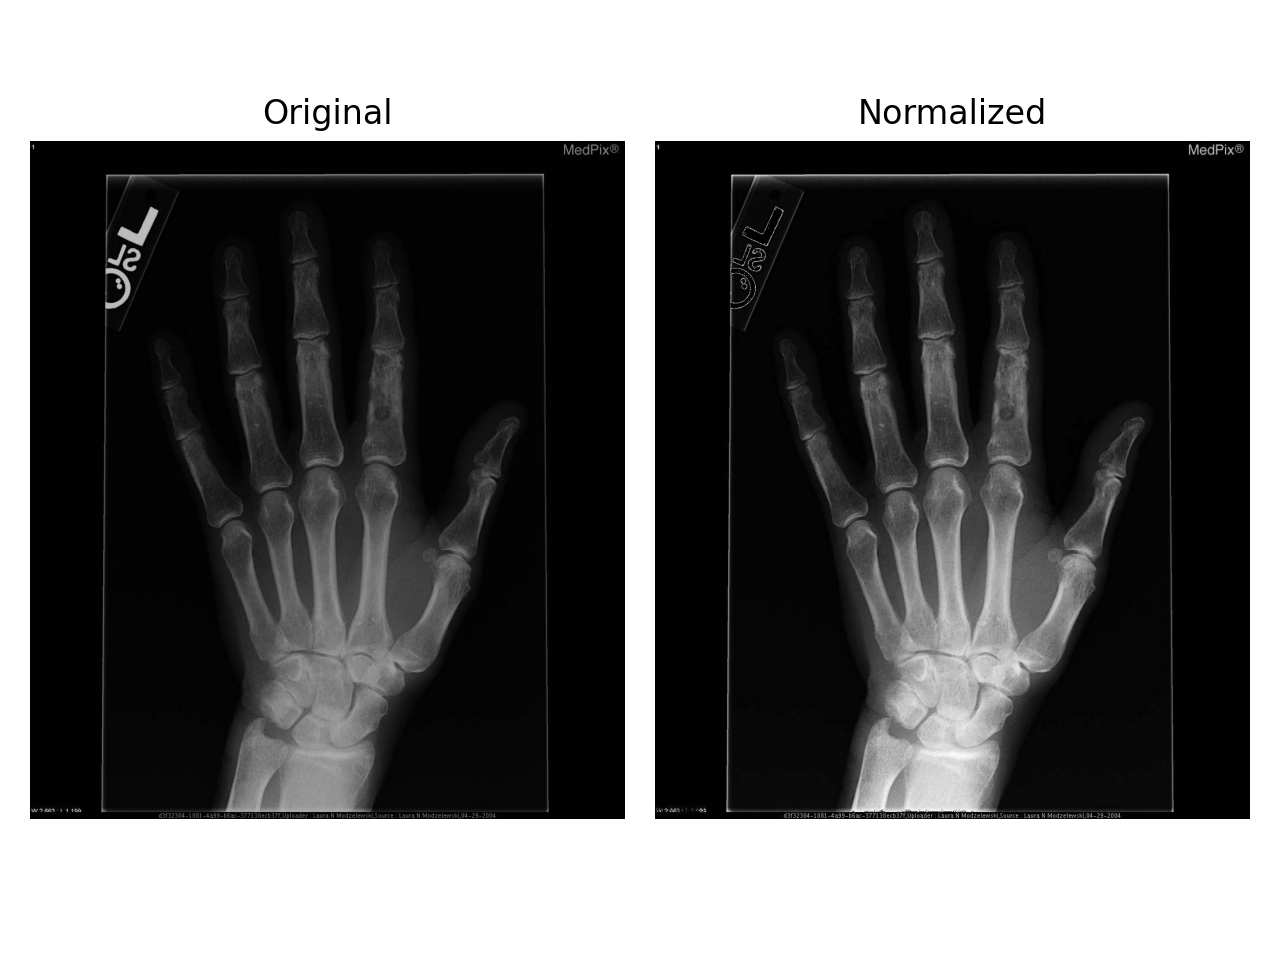
\includegraphics[width=10cm]{pixel_normalization}}
  \caption{Effects of pixel normalization (contrast stretching).}
  \label{fig:pixel_normalization}
\end{figure}

\section{Gamma correction}

\begin{itemize}
\item Corrects for the fact that displays (monitors, projectors, etc.) and
human vision do not respond linearly to intensity values.

\begin{equation}
s = c \cdot r^{\gamma}
\end{equation}

Where:
\begin{itemize}
    \item $r$ = input pixel intensity (normalized to $[0,1]$)
    \item $s$ = output pixel intensity (normalized to $[0,1]$)
    \item $c$ = normalization constant (often $1$)
    \item $\gamma$ = gamma value (controls brightness/contrast)
\end{itemize}

\begin{figure}[H]
  \vspace{-0ex}
  \centering
  \href{https://github.com/vicente-gonzalez-ruiz/medical_imaging/blob/main/notebooks/gamma_correction.ipynb}{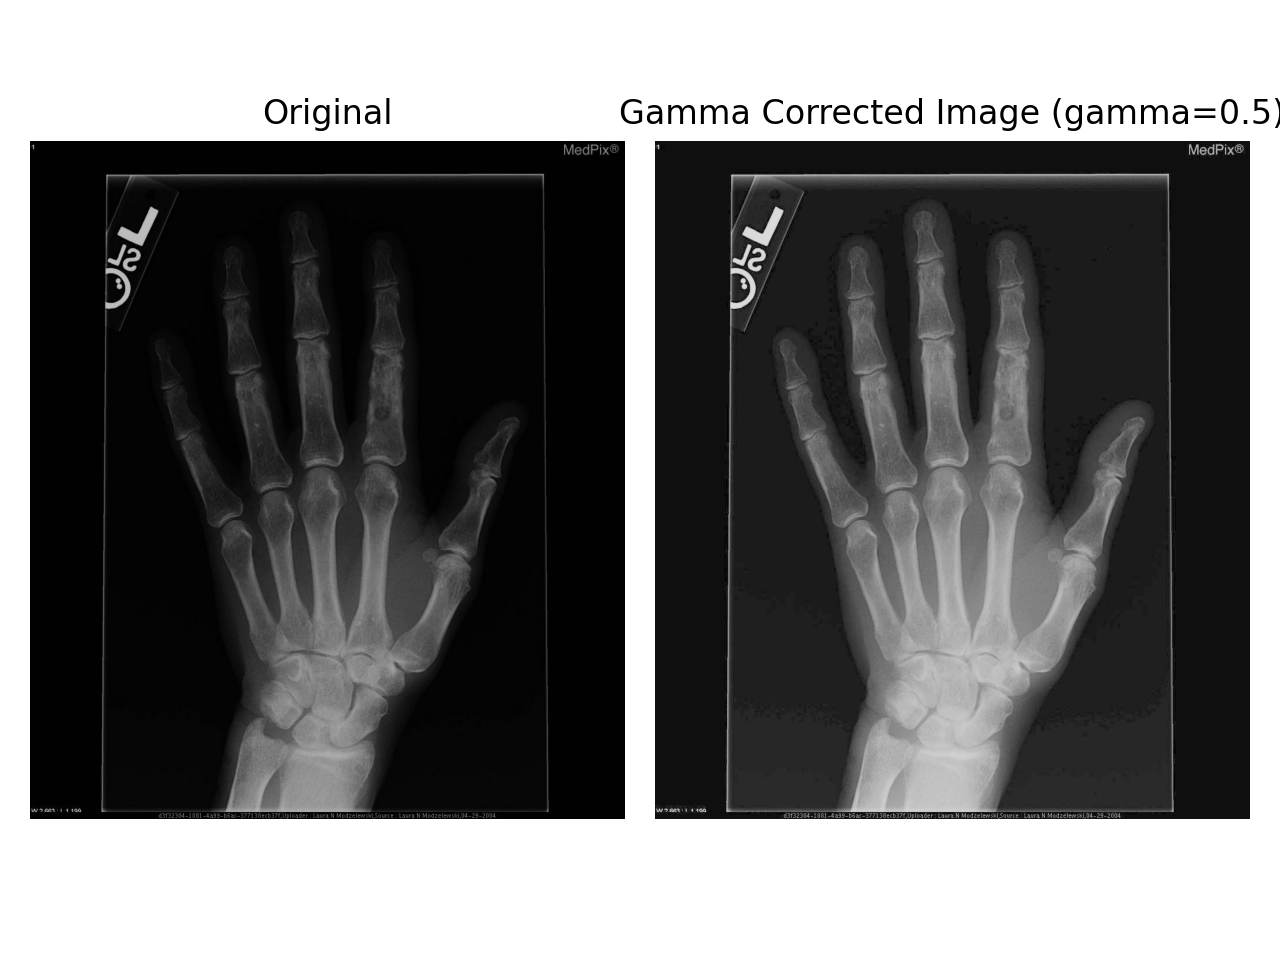
\includegraphics[width=10cm]{gamma_correction}}
  \caption{Effects of gamma correction.}
  \label{fig:gamma correction}
\end{figure}

\end{itemize}


\section{Histogram equalization}

\begin{itemize}
\item Histogram equalization \cite{gonzalez2009digital}
  redistributes the intensity values of an image so that the histogram
  (distribution of pixel intensities) becomes more uniform.
\item The goal is to increase the overall contrast, especially in
  areas that are too dark or too bright.

% Histogram Equalization Formulation
Let an image have $L$ intensity levels $0, 1, 2, \dots, L-1$.

1. Probability of intensity $r_k$:
\[
p(r_k) = \frac{n_k}{N}
\]
where 
\begin{itemize}
    \item $n_k$ = number of pixels with intensity $r_k$
    \item $N$ = total number of pixels in the image
\end{itemize}

2. Cumulative distribution function (CDF):
\[
c(r_k) = \sum_{j=0}^{k} p(r_j)
\]

3. Mapping to new intensity:
\[
s_k = (L-1) \cdot c(r_k)
\]
where 
\begin{itemize}
    \item $r_k$ = original intensity
    \item $s_k$ = new intensity after histogram equalization
\end{itemize}

\begin{figure}[H]
  \vspace{-0ex}
  \centering
  \href{https://github.com/vicente-gonzalez-ruiz/medical_imaging/blob/main/notebooks/equalized_histogram.ipynb}{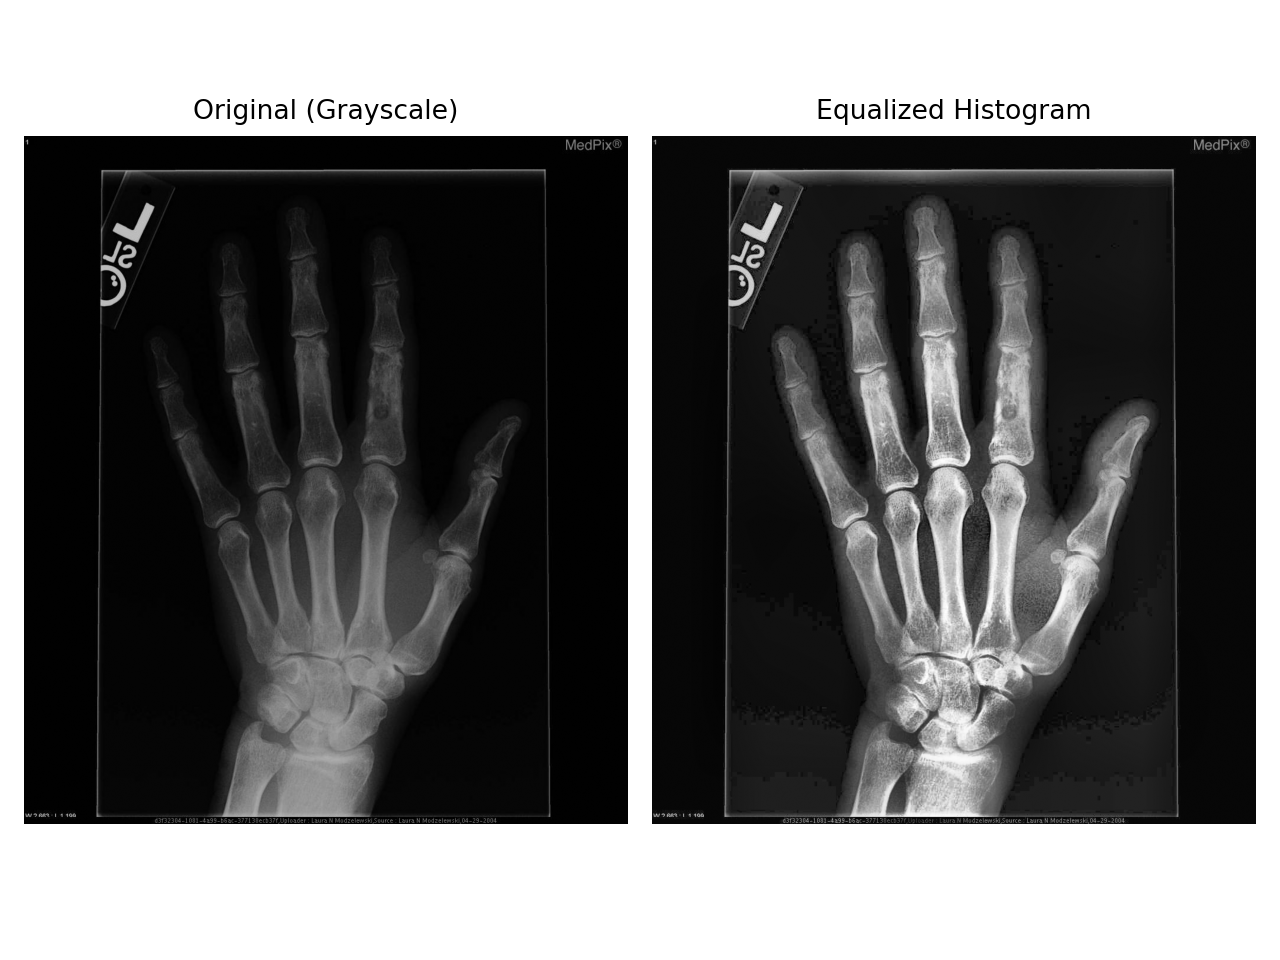
\includegraphics[width=10cm]{equalized_histogram}}
  \caption{Effects of histogram equalization.}
  \label{fig:histogram_equalization}
\end{figure}

\end{itemize}

%section{Sharpening}

\section{Homomorphic filtering \cite{gonzalez2009digital}}

% Homomorphic Filtering Formulation
\begin{itemize}
\item An image can be modeled as the product of illumination and
  reflectance \cite{wikipedia_luminance}:
\[
f(x, y) = i(x, y) \cdot r(x, y)
\]
where
\begin{itemize}
    \item $f(x, y)$ = observed image intensity
    \item $i(x, y)$ = illumination component (slow-varying, low-frequency)
    \item $r(x, y)$ = reflectance component (details, high-frequency)
\end{itemize}

\textbf{Step 1: Logarithmic transformation}
\[
\ln f(x, y) = \ln i(x, y) + \ln r(x, y)
\]

\textbf{Step 2: Fourier transform}
\[
F(u, v) = \mathcal{F}\{\ln f(x, y)\} = I(u, v) + R(u, v)
\]

\textbf{Step 3: Apply a high-pass filter}
\[
S(u, v) = H(u, v) \cdot F(u, v)
\]
where $H(u,v)$ is the filter transfer function.

\textbf{Step 4: Inverse Fourier transform}
\[
s(x, y) = \mathcal{F}^{-1}\{S(u, v)\}
\]

\textbf{Step 5: Exponential transform to restore the image}
\[
f_{\text{enhanced}}(x, y) = \exp(s(x, y))
\]

\begin{figure}[H]
  \vspace{-0ex}
  \centering
  \href{https://github.com/vicente-gonzalez-ruiz/medical_imaging/blob/main/notebooks/homomorphic_filtering.ipynb}{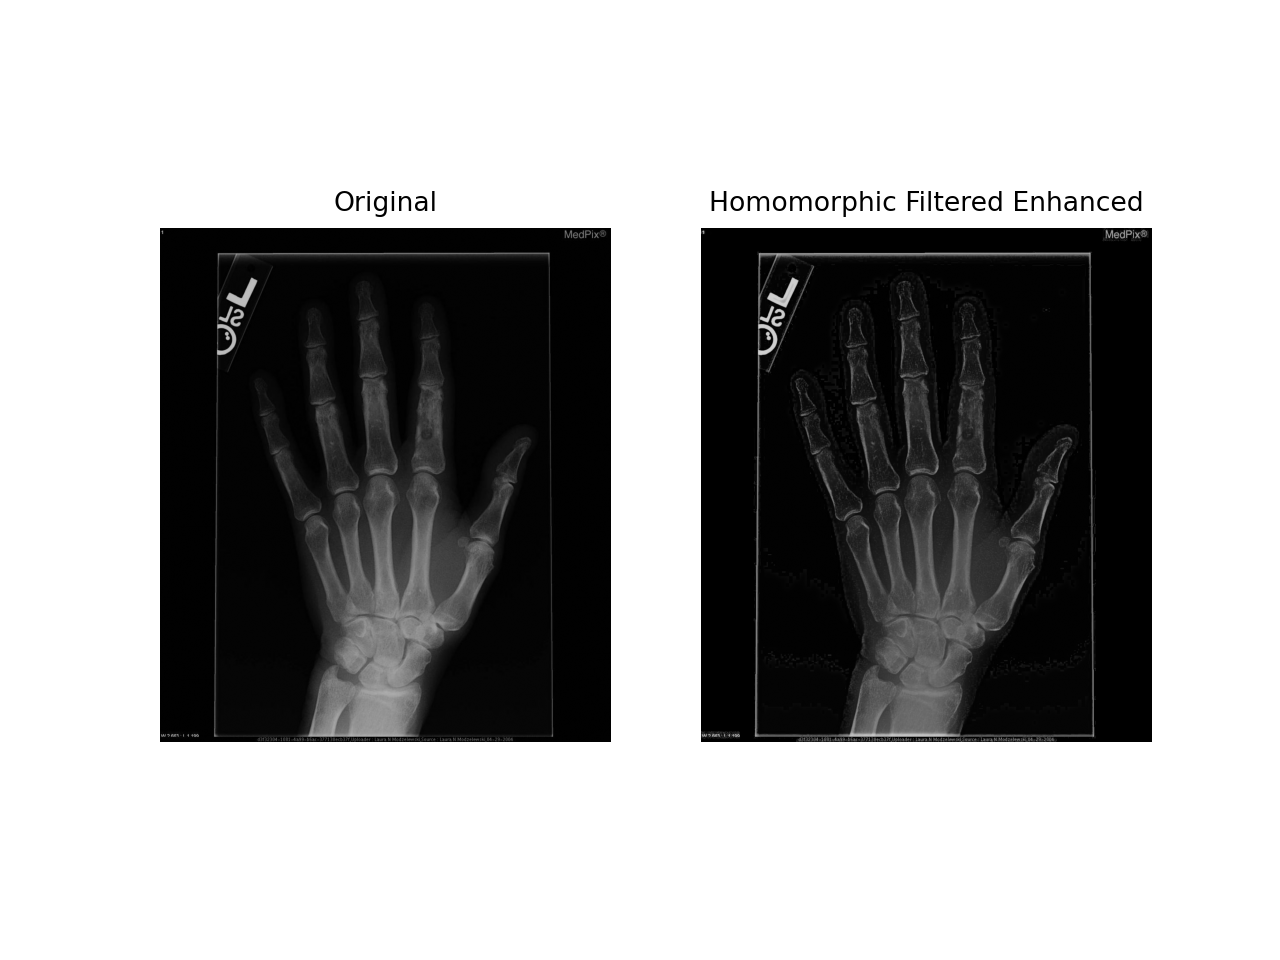
\includegraphics[width=10cm]{homomorphic_filtering}}
  \caption{Effects of homomorfic enhancement.}
  \label{fig:homomorphic_filtering}
\end{figure}

\end{itemize}
